\begin{center}
\vspace{-0.4cm}
\centering
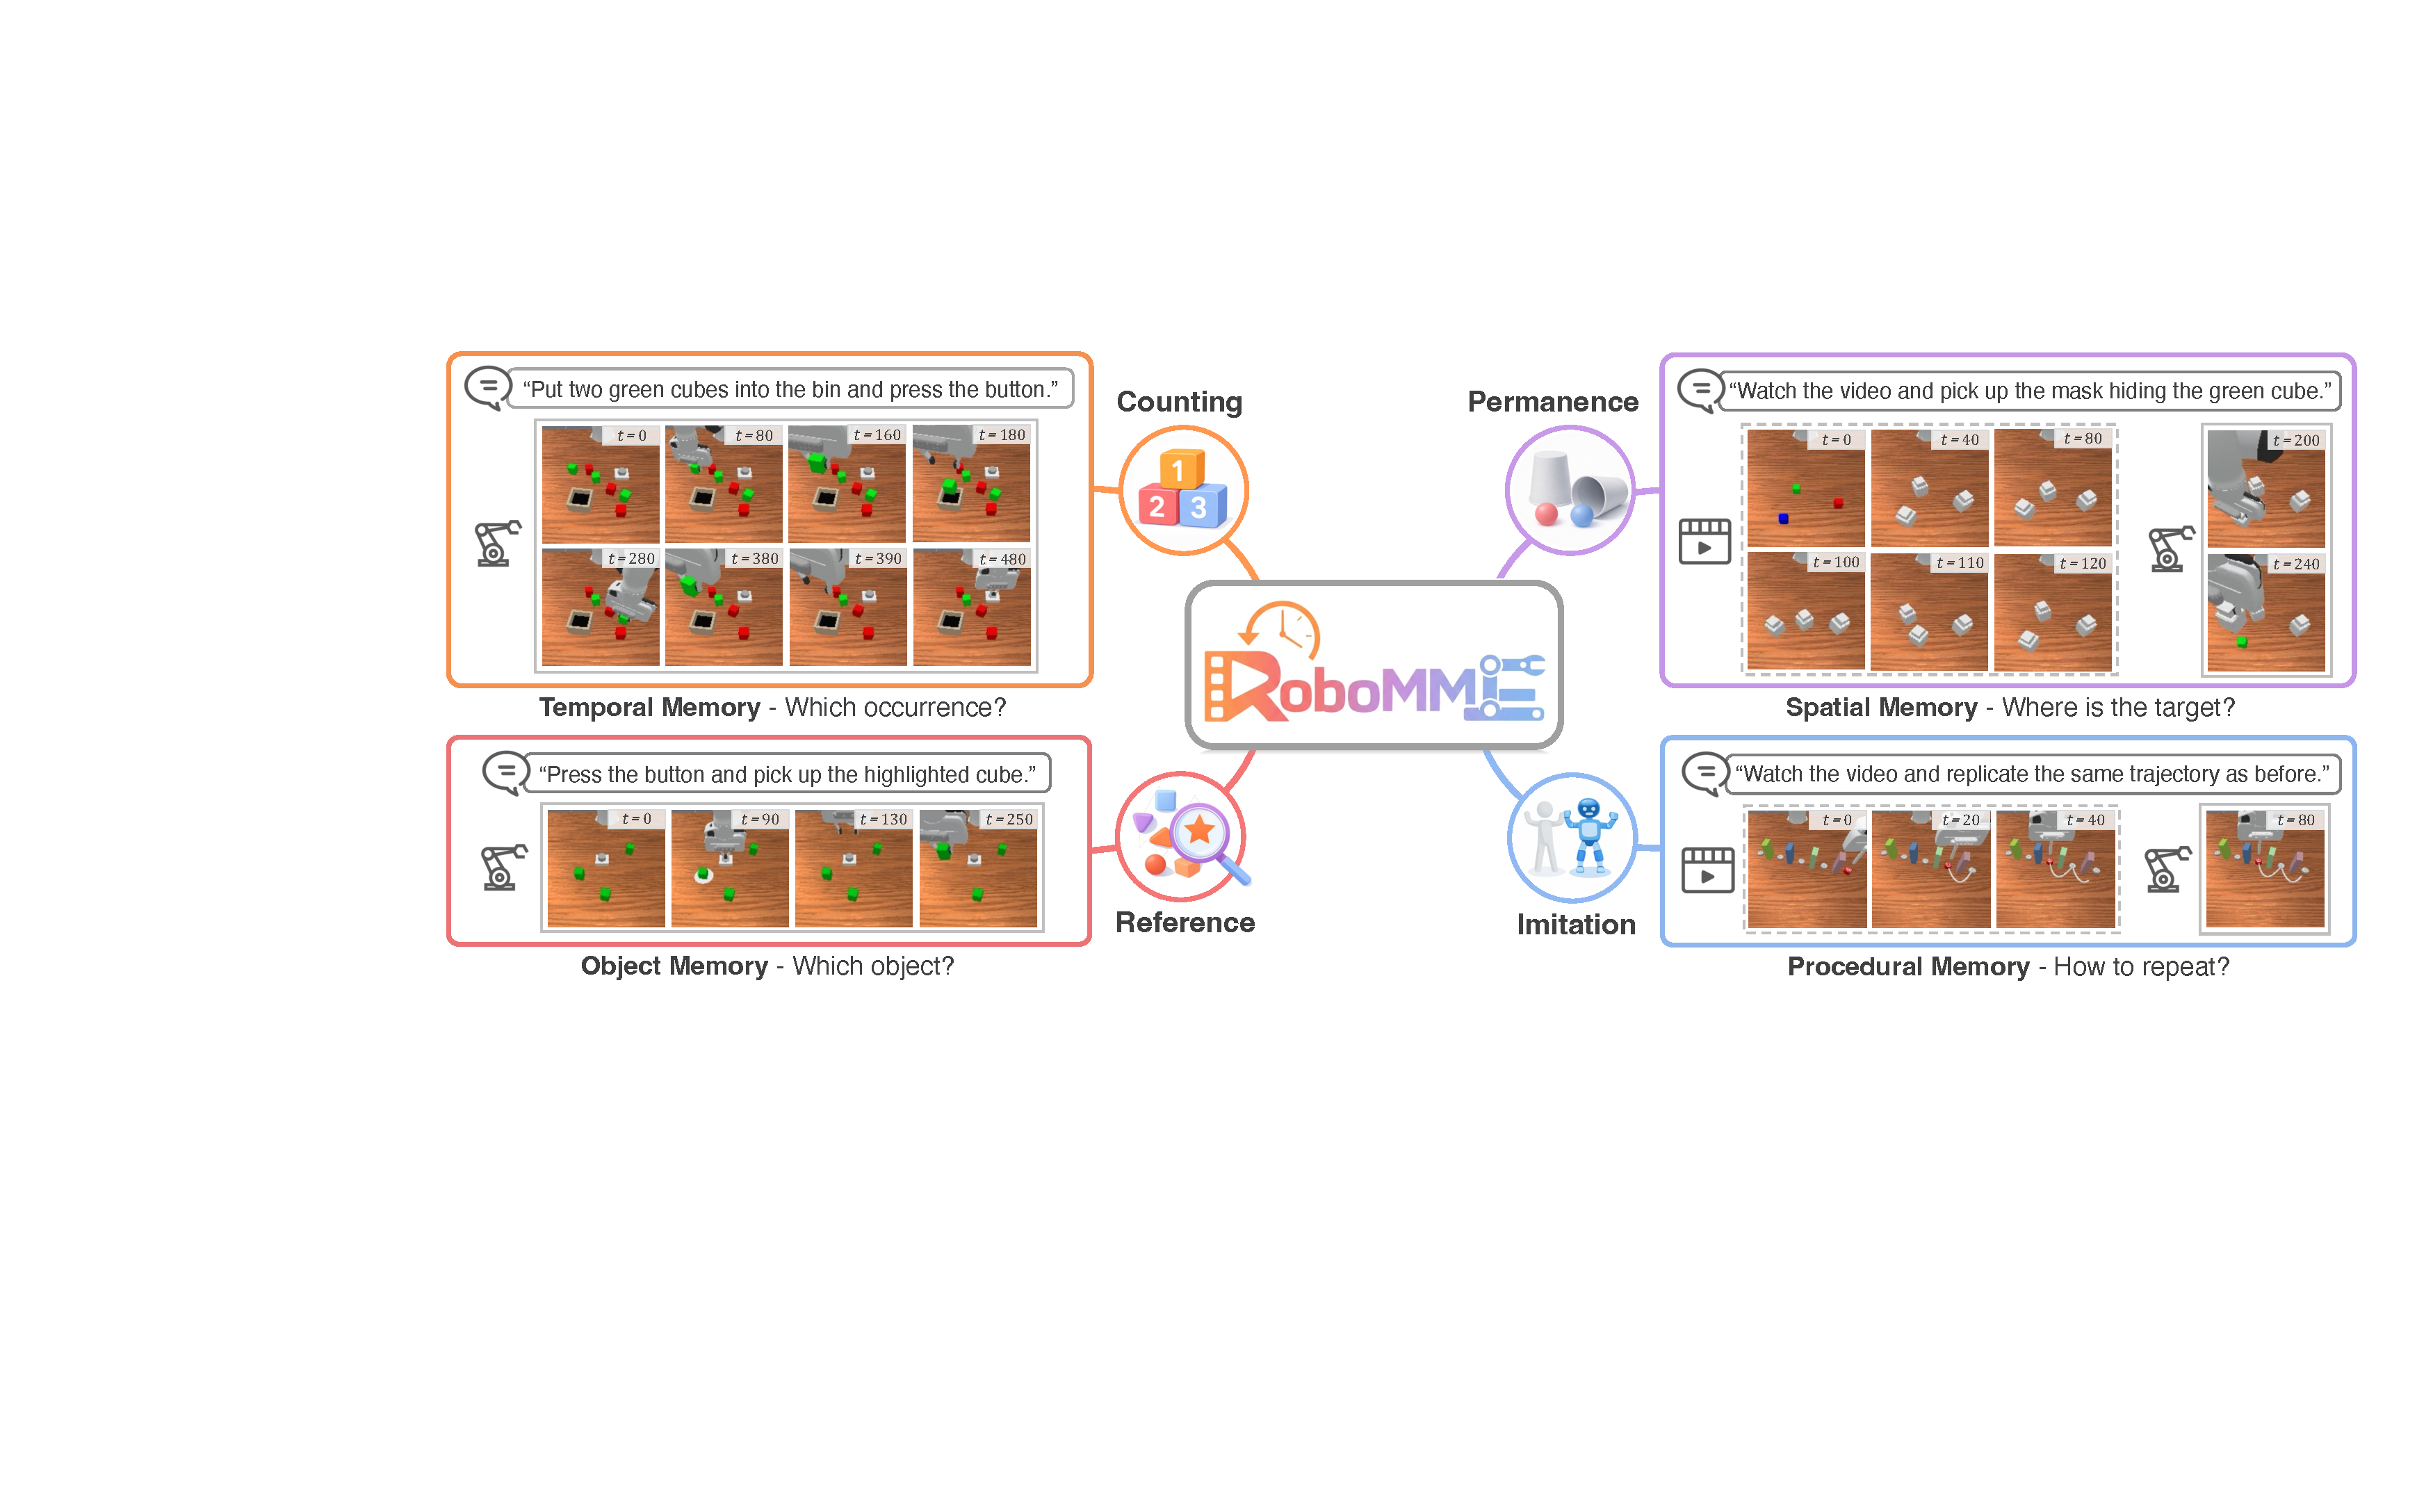
\includegraphics[width=\textwidth]{images/robomme_bench.pdf}
\refstepcounter{figure}
\label{fig:teaser}
\noindent
\begin{minipage}{0.99\textwidth}
    \footnotesize \textbf{Figure~1.} \textbf{\benchname}\xspace is a large-scale robotic benchmark for evaluating memory-augmented manipulation, comprising four task suites that emphasize distinct memory demands.
(1) The \TSone\xspace suite targets \textit{temporal memory}, requiring robots to accumulate and reason over past events, e.g., counting placed green cubes and stopping correctly (top-left).
(2) The \TStwo\xspace suite focuses on \textit{spatial memory}, requiring tracking of object locations under occlusion and environmental changes, e.g., resolving the correct mask after green and blue cubes swap positions (top-right).
(3) The \TSthree\xspace suite evaluates \textit{object memory}, requiring identification under varied referential cues, e.g., recalling a briefly highlighted cube during a button press (bottom-left).
(4) The \TSfour\xspace suite assesses \textit{procedural memory}, measuring the ability to reproduce previously demonstrated behaviors, e.g., replicating a demonstrated trajectory (bottom-right).
Overall, \benchname\xspace includes 16 tasks with \trainsteps\xspace high-quality training timesteps for systematic evaluation of memory-augmented policies.
\end{minipage}
\vspace{0.2cm}
\end{center}

